\documentclass[]{article}
\usepackage{lmodern}
\usepackage{amssymb,amsmath}
\usepackage{ifxetex,ifluatex}
\usepackage{fixltx2e} % provides \textsubscript
\ifnum 0\ifxetex 1\fi\ifluatex 1\fi=0 % if pdftex
  \usepackage[T1]{fontenc}
  \usepackage[utf8]{inputenc}
\else % if luatex or xelatex
  \ifxetex
    \usepackage{mathspec}
  \else
    \usepackage{fontspec}
  \fi
  \defaultfontfeatures{Ligatures=TeX,Scale=MatchLowercase}
\fi
% use upquote if available, for straight quotes in verbatim environments
\IfFileExists{upquote.sty}{\usepackage{upquote}}{}
% use microtype if available
\IfFileExists{microtype.sty}{%
\usepackage{microtype}
\UseMicrotypeSet[protrusion]{basicmath} % disable protrusion for tt fonts
}{}
\usepackage[margin=1in]{geometry}
\usepackage{hyperref}
\hypersetup{unicode=true,
            pdftitle={A national, multi-decadal, water quality and Landsat dataset},
            pdfauthor={Matthew Ross and lots of others!},
            pdfborder={0 0 0},
            breaklinks=true}
\urlstyle{same}  % don't use monospace font for urls
\usepackage{graphicx,grffile}
\makeatletter
\def\maxwidth{\ifdim\Gin@nat@width>\linewidth\linewidth\else\Gin@nat@width\fi}
\def\maxheight{\ifdim\Gin@nat@height>\textheight\textheight\else\Gin@nat@height\fi}
\makeatother
% Scale images if necessary, so that they will not overflow the page
% margins by default, and it is still possible to overwrite the defaults
% using explicit options in \includegraphics[width, height, ...]{}
\setkeys{Gin}{width=\maxwidth,height=\maxheight,keepaspectratio}
\IfFileExists{parskip.sty}{%
\usepackage{parskip}
}{% else
\setlength{\parindent}{0pt}
\setlength{\parskip}{6pt plus 2pt minus 1pt}
}
\setlength{\emergencystretch}{3em}  % prevent overfull lines
\providecommand{\tightlist}{%
  \setlength{\itemsep}{0pt}\setlength{\parskip}{0pt}}
\setcounter{secnumdepth}{0}
% Redefines (sub)paragraphs to behave more like sections
\ifx\paragraph\undefined\else
\let\oldparagraph\paragraph
\renewcommand{\paragraph}[1]{\oldparagraph{#1}\mbox{}}
\fi
\ifx\subparagraph\undefined\else
\let\oldsubparagraph\subparagraph
\renewcommand{\subparagraph}[1]{\oldsubparagraph{#1}\mbox{}}
\fi

%%% Use protect on footnotes to avoid problems with footnotes in titles
\let\rmarkdownfootnote\footnote%
\def\footnote{\protect\rmarkdownfootnote}

%%% Change title format to be more compact
\usepackage{titling}

% Create subtitle command for use in maketitle
\newcommand{\subtitle}[1]{
  \posttitle{
    \begin{center}\large#1\end{center}
    }
}

\setlength{\droptitle}{-2em}

  \title{A national, multi-decadal, water quality and Landsat dataset}
    \pretitle{\vspace{\droptitle}\centering\huge}
  \posttitle{\par}
    \author{Matthew Ross and lots of others!}
    \preauthor{\centering\large\emph}
  \postauthor{\par}
      \predate{\centering\large\emph}
  \postdate{\par}
    \date{20 September, 2018}

\usepackage{booktabs}
\usepackage{longtable}
\usepackage{array}
\usepackage{multirow}
\usepackage[table]{xcolor}
\usepackage{wrapfig}
\usepackage{float}
\usepackage{colortbl}
\usepackage{pdflscape}
\usepackage{tabu}
\usepackage{threeparttable}
\usepackage{threeparttablex}
\usepackage[normalem]{ulem}
\usepackage{makecell}

\begin{document}
\maketitle

{
\setcounter{tocdepth}{2}
\tableofcontents
}
\hypertarget{introduction}{%
\section{Introduction}\label{introduction}}

The production of and easy access to water quality data is a vital first
step towards both understanding the natural and anthropogenic drivers of
water quality variation and for using this knowledge to protect and
manage inland water quality (Srebotnjak et al., 2012). Collecting such
valuable data has historically been expensive, time-consuming, and
difficult to maintain useable and open datasets. However in many
developed nations, over the last 10-20 years many of these data access
problems have been actively addressed leading to the publication and
maintenance of large open-access data repositories on water quality
(Read et al., 2017; Soranno et al., 2017). However, these datasets are
still limited to the relatively time-intensive process of field
sampling, which limits the number of water-bodies that can be observed
and the spatial variation in water quality captured within a single
waterbody. Furthermore, many nations may not have access to such robust
historic water quality sampling data. One way to augment these
\emph{in-situ} sampling efforts and to provide water quality informatino
in places with no data, is through using satellite remote sensing
detection of water quality parameters.

Since the beginning of the Landsat missions, limnologists,
oceanographers, and hydrologists have been interested in developing
universal algorithms for extracting water quality information from
remotely sensed images (Clarke et al., 1970; Holyer, 1978; Klemas et
al., 1973; Maul \& Gordon, 1975; Ritchie et al., 1976). Since these
early efforts there has been almost fifty years of work with the basic
goal of using spectral information to predict water quality parameters
like total suspended solids (TSS), Chlorophyll a (Chl\_a), colored
dissolved organic matter, and secchi disk depth (SDD). However, progress
towards universal algorithms and unified approaches has been slow
(Blondeau-Patissier et al., 2014; Bukata, 2013; Gholizadeh et al.,
2016), with most papers published focusing on developing predictive
methods as opposed to using predictions to interrogate process that
control water quality dynamics {[}Topp2018{]}. Much of this slow
evolution in methods and approaches comes from the inherent optical
complexity of inland waters, where spectral signatures are the result of
a complex mixture of inorganic sediment, organic sediment, algae,
dissolved organic matter, and other constituents. Compared to oceanic
remote sensing of water quality which benefits from robust, shared
datasets of \emph{in-situ} data paired with satellite overpass
reflectance (Blondeau-Patissier et al., 2014; Bukata, 2013), progress on
inland water algorithms is further impeded by the lack of a shared
overpass dataset.

Such data could go a long way towards, if not the holy-grail of
universal predictive algorithms, at least towards more unified
approaches tested on a universal dataset. Here, we create and share the
largest such overpass dataset ever assembled for inland waters by using
Google Earth Engine (Gorelick et al., 2017) Landsat archive data from
1984-2018 with data from the Water Quality Portal (Read et al., 2017)
and phase one of the ``lake multi-scaled geospatial and temporal
database (LAGOS-NE)''(Soranno et al., 2017) for the conterminous USA and
Alaska. Joining these datasets provides us with an unprecedented
resource to model, predict, and understand the long-term and large-scale
dynamics of variation in four key water clarity constituents: TSS, SDD,
Chl\_a, and dissolved organic carbon (DOC). We also outline and share
our approach, code, and intermediate data for bringing these three free
datasets together; generating a high-graded analysis-ready dataset for
remote sensors of water quality.

\#Methods

\hypertarget{parameter-description}{%
\subsection{Parameter description}\label{parameter-description}}

For this project we chose to work with the four most common water
quality parameters used in remote sensing of water quality
{[}Topp2018{]}. All four of these parameters provide useful and
complimentary information on the water quality status of a waterbody and
are also optically active, making them observable from space. Total
Suspended Solids (TSS) is a measure of the mass of solids, both organic
and inorganic, in a watercolumn. TSS scatters light such that generally
more TSS means more light reflected back to the atmosphere and satellite
sensor (Ritchie et al., 1976). Knowing TSS concentrations can provide
insight into light conditions (Julian et al., 2008), erosion conditions
{[}Syvitski2011{]}, and the hydrologic status of waterbody, where high
TSS generally means high flow state (Williams, 1989). Dissolved Organic
Carbon (DOC) is the broad description for the total amount of organic
Carbon that is dissolved in water, and can provide insight into light
conditions (Vähätalo et al., 2005), heterotrophic energy availability
(Robbins et al., 2017), and terrestrial organic matter processing
(Williamson et al., 2008). While DOC does not inherently alter the
optical properties of water, it is generally strongly correlated with
Colored Dissolved Organic Matter (CDOM), which is optically active,
generally a brown color (Griffin et al., 2011). For this project, we
downloaded both DOC and CDOM data. Chlorophyll a is photosynthetically
active pigment contained in all phytoplankton, which helps give algal
blooms their green color. Chlorophyll a concentrations can be used to
detect algae blooms (Kutser, 2004), estimate primary productivity
(Antoine et al., 1996), and understand algae dynamics (Richardson,
1996). Finally, we gathered data on secchi disk depth, which is a method
for estimating water clarity that dates back to 1864 (Secchi, 1864). The
secchi disk is a 30 cm diameter disk divided into four quadrants painted
altertanitively white and black. To measure water clarity, this disk is
lowered into a waterbody, and the depth at which the disk is no longer
visible is called the secchi disk depth. Deeper depths mean clearer
water. Secchi disk depth is an easy measurement to make that integrates
the optical properties of all water constituents and can provide
information on the trophic status of waterbodies (Carlson, 1977), the
algae status of a waterbody (Lorenzen, 1980), and many other uses. These
four parameters capture key ecological and physical factors that control
water quality and have a robust literature demonstrating the ability to
remotely sense each constituent {[}Topp2018{]}, making them ideal for
our dataset construction efforts.

\hypertarget{data-source-description}{%
\subsection{Data source description}\label{data-source-description}}

Combining \emph{in-situ} data with Landsat reflectance information first
requires a large repository of water quality samples, which increases
the likelihood that a given sample happened to be taken on the same day
as a Landsat overpass. For this paper, we focused on two databases of
water quality. The first, the Water Quality Portal (WQP) has tens of
millions of water observations in all types of inland surface waters,
but there is no entity that harmonizes and cleans the data for quality
(Read et al., 2017). The second dataset we used, LAGOS, currently only
covers lakes in the northeastern United States, with plans to expand and
cover lakes across the entire USA (Soranno et al., 2017). While LAGOS
has less data than the WQP, a group of dedicated researchers has spent
years combing through the data and ensuring data quality, making it a
more analysis-ready dataset (Soranno et al., 2017). These similar but
contrasting datasets, one with more quantity (WQP) and the other with
more quality assurances (LAGOS), ensures that our dataset covers the
broadest possible number of waterbodies with the option of limiting
analyses to only the highest quality subset.

\hypertarget{water-quality-portal}{%
\subsubsection{Water Quality Portal}\label{water-quality-portal}}

The WQP is the largest dataset of water observations ever assembled with
more than 290 million observations at 2.7 millions sites mostly in the
USA, with data dating back more than a century (Read et al., 2017). The
WQP continuously gathers water quality information from more than 450
organizations including academic, government, NGO, tribal, and state
datasets (Read et al., 2017). These datastreams are gathered and
distributed in a standardized format, making analysis across different
collection methods more readily available. Yet, the diversity of data
sources and variation in meta-data quality brings about some significant
challenges to directly using the WQP as a analysis-ready dataset
(Sprague et al., 2017). Instead end-users of the data must carefully
harmonize data across sampling methods, analytic approaches, and units.
The nature of harmonizing such large, distributed data generates a
necessary trade-off between a deep, time-consuming exploration of data
interoperability and a more shallow less time-consuming but potentially
more error-prone data quality check.

\hypertarget{lagos-ne}{%
\subsubsection{LAGOS-NE}\label{lagos-ne}}

The LAGOS project was, in part, meant as a direct way to address some of
the problems inherent to the WQP, with the explicit goal of building a
publically available high-quality dataset for continental-scale lake
analyses (Soranno et al., 2017). In addition to pairing \emph{in-situ}
lake data with physical lake characteristics and local geologic setting,
LAGOS researchers standardized key water quality measurements across the
87 water quality datasets that they gathered (Soranno et al., 2017).
Because LAGOS harmonized data from many different sources, they chose to
identify all data for a single lake with the lake centroid. So, if two
different organizations were measuring secchi disk depth at the north
and south end of a lake, the LAGOS dataset would combine all these
measurements into a single lake centroid estimate. This lake centroid
approach is differnt from the data in the Water Quality Portal and
should be kept in mind throughout this paper. In it's current form, the
LAGOS dataset covers only lakes in the northeast and midwest, two
lake-rich regions of the USA. LAGOS provides an end-member dataset of
the highest quality for matching \emph{in-situ} data to Landsat
overpasses.

\hypertarget{landsat}{%
\subsubsection{Landsat}\label{landsat}}

For this project, we join these two \emph{in-situ} datasets with the
Landsat data archive for Landsat missions 5, 7, and 8. The Landsat
missions started in July 1972, as the Earth Resources Observation
Satellite with an explicit mission to provide solutions for some of
earth's pressing issues associated with industry and environmental
change (Loveland \& Dwyer, 2012). For this project we are only using the
three most recent Landsat mission datasets: Landsat 5 with coverage from
1984-2012 and over 192745 available images; Landsat 7 which is still
collecting data after launching in July of 1999 with 191366 images; and
finally Landsat 8 which launched in November, 2013 still adding to its
collection of 61790 images. The total usable images will be much less
than the total images because of cloud cover, which varies greatly by
region. Furthermore, on May 31, 2003, the Landsat 7 scan line corrector
failed, causing the Landsat 7 images after this date to have striped
data gaps (Storey et al., 2005). For our purposes, we kept all Landsat 7
data after this date, but did no gap-filling, such that if a site were
entirely situated in a gap, it would report no Landsat 7 data.
Generally, these satellites complete a full imaging of the globe every
sixteen days, except for the most polar regions (Loveland \& Dwyer,
2012; Wulder et al., 2016), meaning that for most of the USA, a given
spot will be imaged at least every sixteen days, and-when two missions
are running at the same time- every eight days. All three satellites use
different imagers to collect spectral information in the visible and
infrared wavelengths at 30 meter resolution pixels.

\hypertarget{data-integration}{%
\subsection{Data integration}\label{data-integration}}

For this project, we wanted to emphasize not only the possibilities that
come with open data, but also the importance of reproducible science and
code. In this case uniting these three distinct datasets requires a
combination of computational approaches and an architecture that allows
for a single workflow to pull data from LAGOS, the WQP, and the Landsat
archive. Despite such disparate data sources, an ideal overarching
approach allows us to break the various data pulls, munging, and joining
into seperate pieces that can be updated only as needed. Here we chose
to use a ``MAKE'' like environment (Feldman, 1979) that only executes
sections of code that have been altered or when data sources are out of
date. Though this project uses three different tools R, Python, and
Google Earth Engine, all of these various languages are called directly
from R and RMarkdown files. This reliance on R makes remake
\url{https://github.com/richfitz/remake} an excellent choice to keep
track of changes to the complex commands required to compile this
dataset. Remake provides an R specific MAKE-like environment that can
check if code has been updated and then update all downstream data. We
hope that these efforts will make recreating or altering our specific
approach easier. At a high level, all of this architecture is meant to
do something fairly simple captured by figure \ref{fig:fig1}, joining
\emph{in-situ} data to Landsat reflectance.

\begin{figure}
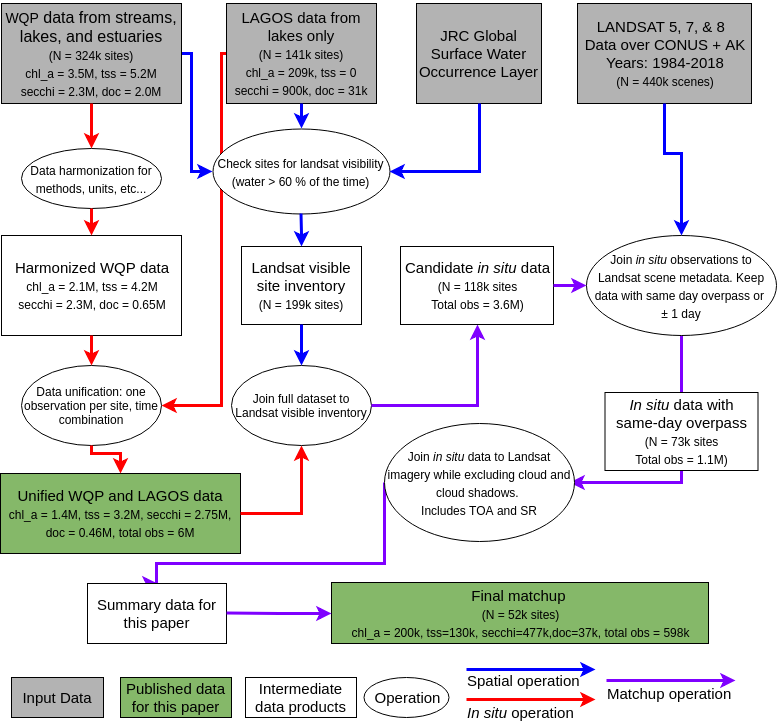
\includegraphics[width=0.8\linewidth]{C:/Users/mrvr/Dropbox/UNC-PostDocAll/aquasat/4_report/src/Watersat_Drop_flow} \caption{Overview of data sources, steps taken to join data, and total observation counts}\label{fig:fig1}
\end{figure}

\hypertarget{in-situ-data-pull-and-quality-control.}{%
\subsubsection{\texorpdfstring{\emph{In situ} data pull and quality
control.}{In situ data pull and quality control.}}\label{in-situ-data-pull-and-quality-control.}}

In this paper we focused on gathering water quality measurements that
capture the dominant controls on water clarity, these include:
Chlorophyll a (Chl\_a), dissolved organic carbon (DOC), and total
suspended solids (TSS). Together these three constituents combine with
other optically active solutes and solids to control total water clarity
which is captured by secchi disk depth measurements, the fourth and
final parameter we pulled for these analyses. For the WQP we used the
\href{https://github.com/USGS-R/dataRetrieval}{dataRetrieval} package.
DataRetrieval, a package maintained and supported by the USGS, allows
for programattically downloading data from the WQP. The WQP contains
hundreds of possible paramater types (called ``characteristicName'' in
the WQP), and we carefully selected those that best represented our
target parameters based on our own expertise and previously published
research using the same data sources(Butman et al., 2016; Stets \&
Striegl, 2012). The characteristicName's that we pulled are shown in
table \ref{tab:table1}. For all parameters, we pulled data for all US
states. The WQP classifies water body types in many possible categories
and we pulled data for the four following water body types: Lake,
Reservoir, Impoundment; Stream; Estuary; Facility. Finally, we only
gathered data that was reported to have been sampled in ``Water'' as a
sample media (no sediment or benthic samples).

Working with the LAGOS-NE data (version 1.087.1) required many less
decisions to combine parameters since LAGOS researchers have already
harmonized and combined parameters into simple categories that reflect
our general parameter codes(Soranno et al., 2017). LAGOS includes lake
data for: DOC, Chlorophyll a, and secchi disk depth, but no data on TSS.
As with the WQP the dataset can be simply loaded using an R package
(`LAGOS-NE')(Soranno et al., 2017). This clean dataset requires very
little data cleaning and was essentially preserved as a direct product
from the LAGOS-NE dataset, in sharp contrast to the much more intensive
data cleaning required to use the WQP data.

\rowcolors{2}{gray!6}{white}
\begin{table}

\caption{\label{tab:table1}Table shows the characterstic names used in our water quality portal data pull.}
\centering
\begin{tabular}[t]{>{\raggedright\arraybackslash}p{2cm}|>{\raggedright\arraybackslash}p{13cm}}
\hiderowcolors
\hline
\textbf{Parameter} & \textbf{WQP Names}\\
\hline
\showrowcolors
cdom & Colored dissolved organic matter (CDOM)\\
\hline
chlorophyll & Chlorophyll; Chlorophyll A; Chlorophyll a; Chlorophyll a (probe relative fluorescence); Chlorophyll a (probe); Chlorophyll a - Periphyton (attached); Chlorophyll a - Phytoplankton (suspended); Chlorophyll a, corrected for pheophytin; Chlorophyll a, free of pheophytin; Chlorophyll a, uncorrected for pheophytin; Chlorophyll b; Chlorophyll c; Chlorophyll/Pheophytin ratio\\
\hline
doc & Organic carbon; Total carbon; Hydrophilic fraction of organic carbon; Non-purgeable Organic Carbon (NPOC)\\
\hline
secchi & Depth, Secchi disk depth; Depth, Secchi disk depth (choice list); Secchi Reading Condition (choice list); Secchi depth; Water transparency, Secchi disc\\
\hline
tss & Total suspended solids; Suspended sediment concentration (SSC); Suspended Sediment Concentration (SSC); Total Suspended Particulate Matter; Fixed suspended solids\\
\hline
\end{tabular}
\end{table}
\rowcolors{2}{white}{white}

Turning data from the WQP into an analysis-ready dataset similar to
LAGOS-NE requires a chain of decisions that is extensively documented in
the supplemental \href{link}{website}. We have attempted to make these
decisions both clear and justifiable, with the end goal of having
parameters meet several criteria. First, all observations were verified
to ahve analytical methods that matched their parameter name, if this
were not the case samples were dropped. For example, if an observation
was supposed to report TSS, and the analytical method was ``Nitrogen in
Water,'' then that sample would be dropped. For TSS in particular, we
assumed that the characteristicName Suspended Sediment Concentration
reflected essentially the same data despite some methodoligical
differences in the data as shown
\href{https://water.usgs.gov/osw/pubs/WRIR00-4191.pdf}{here}. Second,
all parameters were checked to make sure that the characteristicName
that was queried, matched the actual parameter of interest that was
downloaded. For example, if we queried ``Dissolved Organic Carbon''
data, but the parameter name in the data was ``Total Organic Carbon''
then we would drop those samples. Third, we harmonized the data across
units such that TSS and DOC data are in mg/L, Chl\_a data is in
\(\mu g/L\), and secchi disk depth is in meters. If units were
nonsensical (secchi in mg/L), then we would drop those observations.
Finally, we forced both the LAGOS-NE and the WQP data to have only one
observation per datetime X site combination. We did this by either
removing true duplicates (where the value was the same for multiple
observations), averaging multiple observations to a single observation
if the coefficient of variation was less than 0.1, and throwing out
observations with too many simultaneous observations (5 per date time
combination) or too much variation with no metadata explaining the
repeat observations. We used a similar procedure for the data that did
not have timestamps and only had date information, these data without
timestamps were set to observations at noon for matching to Landsat
dates. In general, we assume that these simultaneous observations are
either reporting errors, represent field sampling campaigns with
genuinely simultaneous observations, or reflect simultaneous sampling at
different depths. Figure \ref{fig:fig1} captures how these data cleaning
procedures cut out observations and sites.

While our data quality control included many checks to ensure data
quality, we also consciously avoided some other data quality assurance
steps because including them would have thrown out the majority of the
WQP data. For example, some samples included sampling depth information,
which is particularly important when matching water quality data to
reflectance information, but so few samples included depth information,
that we elected to simply keep all the data, assuming that the majority
of the data was collected near the surface (see supplement for
justification of this assumption). Some of these decisions included: not
filtering data based on sampling method, not including temperature data
as a filter for DOC and Chl\_a samples, and including data that had
unlabeled sample fraction metadata. We know that some of these decisions
may not match the requirements of other research, so we have included
code and data that would allow future researchers to choose different
data quality criteria and recreate a similar, more strict dataset.

\hypertarget{joining-in-situ-data-to-landsat}{%
\subsubsection{\texorpdfstring{Joining \emph{in-situ} data to
Landsat}{Joining in-situ data to Landsat}}\label{joining-in-situ-data-to-landsat}}

Because of the 30 m resolution of Landsat, our ability to detect
waterbodies is limited to waterbodies that are wider than at least 60 m
on all sides to ensure that the spectral information captures only
purely water pixels. In essence, this means that our ``Stream'' data is
really limited to relatively large rivers wider than 60 m, though we use
the terms stream and river interchangeably. Similarly, Estuaries and
Lakes are mostly limited to sites that where the waterbody is wider than
60 m.

Both the WQP and LAGOS-NE datasets come with site information that
includes latitude and longitude. Joining the \emph{in-situ} data to
Landsat requires using this location data to select sites, gather
spatially averaged reflectance, and match water quality data
observations to simultaneous overpasses. For the location data, we
encounter an interesting difference in philosophy, where the WQP records
locations at the site of the observation and LAGOS-NE records location
as the center of the lake under observation. This means that if data is
both in the WQP portal and in LAGOS-NE, then we will potentially have
different reflectance information for the same water quality
observation. In the WQP data, where sampling sites are often along the
shores of lakes and banks of rivers, the exact sampling location may be
more likely to include ``spoiled'' pixels that contain some spectral
information of the pure water body and the adjacent land. Keeping sites
pinned to the reported sampling location does allow for more spatial
variation in waterbody water quality, which could reflect genuine
spatial variation in water quality in larger waterbodies (Griffin et
al., 2011). In the LAGOS-NE dataset, using lake centroid spectral
information essentially eliminates the risk of pixel contamination for
most large lakes, but makes the implicit assumption that water quality
does not vary too much across the water body. We kept both of these data
sources, so that data users can choose which data source best suits
their needs.

The first step in linking these datasets is finding out which water
bodies are likely to be Landsat visible, where the 30m resolution pixels
of Landsat detect an unspoiled (entirely water) pixel. We elected to
only keep sites that are not only classified as water some of the time,
but are generally classified as water throughout the Landsat archive
record, using an 80\% threshold on the Pekel occurrence layer (Pekel et
al., 2016). Pekel and others (2016) used the Landsat archive to generate
a global map of how often a given pixel was classified as water from
1985-2015. For our purposes we only kept sites that were within 200
meters of at least one pixel with a water occurence of at least 60\%.
All such sites were kept in the dataset and were sptially joined to an
inventory of landsat overpass path and row, where each site was then
affiliated with a specific landsat tile.

We then generated a dataset that included information on the exact date
and time that any of the three Landsat missions imaged a given tile.
This data was then joined to the \emph{in-situ} observation data by
date. If multiple observations were taken on the same day, we kept only
the observation that was closest in time to the landsat overpass. In
order to maximize the size of the dataset, we also shouldered the
\emph{in-situ} data by one day, allowing for data to be collected
\(\pm\) one day of an overpass. This one-day shouldering is relatively
conservative for previous work in lakes (Olmanson et al., 2011; Torbick
et al., 2013) and rivers (Griffin et al., 2011), but is likely too
permissive for estuaries and rivers with rapidly changing discharge,
where water clarity characteristics vary on sub-hour intervals (Rode et
al., 2016). The timing difference between overpasses and \emph{in-situ}
collection is preserved in the final dataset and users can specify
minimum overpass timing if they choose to be more strict.

With this trimmed down dataset of Landsat-visible sites matched to
Landsat overpass times, we used Google Earth Engine to pair
\emph{in-situ} observations with Landsat reflectance values. Landsat 5
and 7 have onboard imagers that collects seven bands of imagery centered
on three visible wavelengths (blue, green, and red) and four infrared
(near infrared, shortwave infrared 1, shortwave infrared 2, and thermal
band). Landsat 8 has the same bands with slightly different wavelengths
and improved spectral accuracy (Barsi et al., 2014) plus a few extra
bands that we did not include in this work. Landsat 7 and 8 have
panchromatic bands at 15m resolution, while landsat 5 does not. For our
matchup data, the bands we used their wavelengths and resolution are in
table \ref{tab:landsat}.

\rowcolors{2}{gray!6}{white}
\begin{table}

\caption{\label{tab:landsat}Landsat spectral summary}
\centering
\begin{tabu} to \linewidth {>{\raggedright}X>{\raggedright}X>{\raggedright}X>{\raggedright}X>{\raggedright}X}
\hiderowcolors
\hline
\textbf{Bands} & \textbf{L5 Wavelengths} & \textbf{L7 Wavelengths} & \textbf{L8 Wavelengths} & \textbf{Resolution (m)}\\
\hline
\showrowcolors
Blue & 0.45-0.52 & 0.45-0.52 & 0.452-0.512 & 30\\
\hline
Green & 0.52-0.60 & 0.52-0.60 & 0.533-0.590 & 30\\
\hline
Red & 0.63-0.69 & 0.63-0.69 & 0.636-0.673 & 30\\
\hline
Near Infrared (nir) & 0.77-0.90 & 0.77-0.90 & 0.851-0.879 & 30\\
\hline
Shortwave Infrared 1(swir1) & 1.55-1.75 & 1.55-1.75 & 1.566-1.651 & 30\\
\hline
Shortwave Infrared 2 (swir2) & 2.09-2.35 & 2.09-2.35 & 2.107-2.294 & 30\\
\hline
Panchromatic & NA & 0.52-0.9 & 0.503-0.676 & 15\\
\hline
\end{tabu}
\end{table}
\rowcolors{2}{white}{white}

At each site, we generated a 200 m buffer around the site. Within this
buffered zone, we throw out any pixel that is not classified as water at
least 80\% of the time in the landsat archive (Pekel et al., 2016). We
elected to initially only filter sites down to an initial threshold of
60\% in order to include as many sites as possible in the candidate site
pool. At the stage where we are direclty linking reflectance to
\emph{in-situ} concentration, we elected to set a more strict threshold
in order to minimize the likelihood of getting partial or spoiled
pixels. All of the Landsat data comes with quality assessment bands that
indicate if individual pixels are likely taken of land, water, clouds,
aerosols, etc\ldots{} We used these bands to throw out any pixels that
were classified as cloud and cloud shadows, but we elected to keep all
data classified as land, ice, or water, since very high sediment
concentrations can lead to classification as water or ice (Xiao
citation?). In addition to these steps, we also created a 30 m buffer
around the TIGER road
\href{https://www.census.gov/geo/maps-data/data/tiger.html}{dataset}
from the US Census office, all pixels that were within 30m of any
transport artery (road, traintracks, etc\ldots{}) was removed. Once
these extra steps were taken for removing pixels that would likely spoil
the reflectance signal coming from the water, we took a spatial median
of all remaining pixels in the buffer zone for all bands. This spatial
median includes a median of the quality assessment band, which can be
used to indicate if the median assessment value was water or some other
class like land or ice. This step leaves us with a ``wide'' (Wickham,
2014) dataset with the \emph{in-situ} observation values in columns
arranged with reflectance values from landsat for the same site X date
combination.

One of the most critical components of inland water remote sensing is
the atmospheric correction, where radiance at the satellite sensor is
corrected to radiance from the land surface (Brando \& Dekker, 2003;
Caselles \& Lóópez Garc Ĺ A, 1989). Atmospheric correction, when
properly applied can correct for aersol interference, sun glint, and
other processes that might alter the radiance leaving waterbodies,
giving a much cleaner signal of the optical qualities of water (Gordon,
1997). There are many options for atmospheric correction algorithms, but
Google Earth Engine only houses the USGS Surface Reflectance archive
which uses a version of the 6S radiative transfer model called LEDAPS
for Landsat 5 and 7 (Ju et al., 2012). For Landsat 8 the algorithm is
called LaSRC that uses the ultra blue band to correct for aersols
(Doxani et al., 2018). Because the Google Earth Engine archive only
houses this one atmospheric correction approach, we pull both the USGS
surface reflectance and the uncorrected top-of-atmosphere reflectance.
Ideally this allows end users to use their best judgement for which
product is best suited to their needs. At the end of this long chain of
decisions, and operations, we are left with a matchup of dataset of
nearly 600,000 matchups between \emph{in-situ} data and Landsat
reflectance. As far as we know this is the largest such dataset for
inland water quality and some of it's summary features are described
below.

\begin{center}\rule{0.5\linewidth}{\linethickness}\end{center}

\hypertarget{results}{%
\section{Results}\label{results}}

As figure \ref{fig:fig1} shows, matching data to landsat overpasses
generally reduced the total available data for a given paramter by 6-25
times, with the biggest dropoff in TSS observations and the most
retained with secchi disk depth. This intuitively makes sense, as most
TSS observations are made in streams which aren't Landsat visible, while
secchi observations are mostly in lakes, which are visible. As a result
of this steep dropoff we elected to drop CDOM from the pipeline because
there were only 2761 CDOM results in the entire WQP before any data
cleaning. The remaining data is well distributed across the parts of the
USA with many lakes and rivers in the Upper Midwest, Northeast, and
Florida, with notable data concentrations near the Chesepeake Bay and
along the U.S. East Coast in major estuarine environments (Fig
\ref{fig:map}). The western United States has notably less data
available, which likely reflects both much lower concentrations of lakes
and rivers, and potentially a bias in the completeness of the WQP
towards certain states.

\begin{figure}
\centering
\includegraphics{aquasat_outline_files/figure-latex/map-1.pdf}
\caption{\label{fig:map} Distribution of observations across the
conterminous USA. The data is split by observation type, where total
represents an overpass for any of the four primary parameters}
\end{figure}

\begin{figure}
\centering
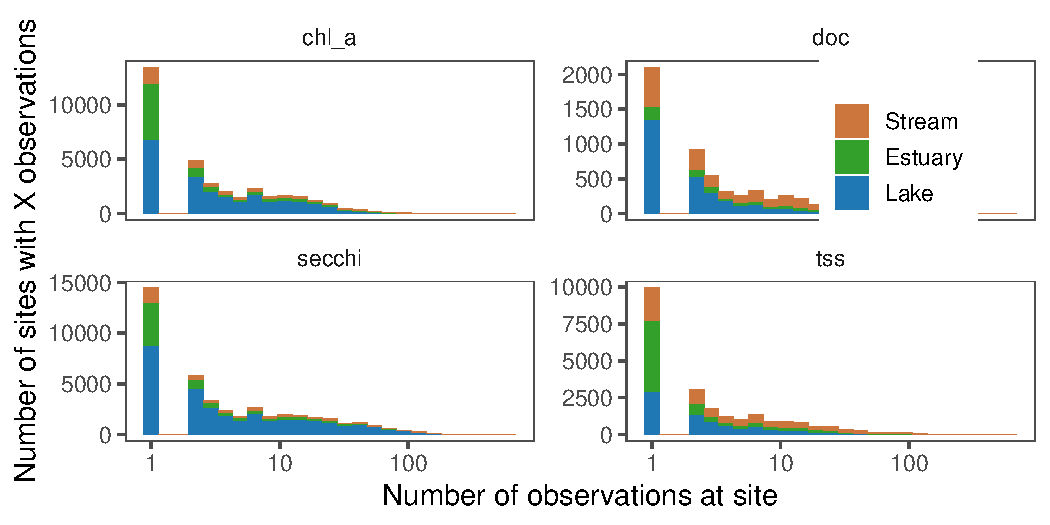
\includegraphics{aquasat_outline_files/figure-latex/distribution-1.pdf}
\caption{\label{fig:distribution} Shows the distribution of observations
at a given site. Most sites only have a single overpass observation, but
there are thousands of these sites}
\end{figure}

\begin{figure}
\centering
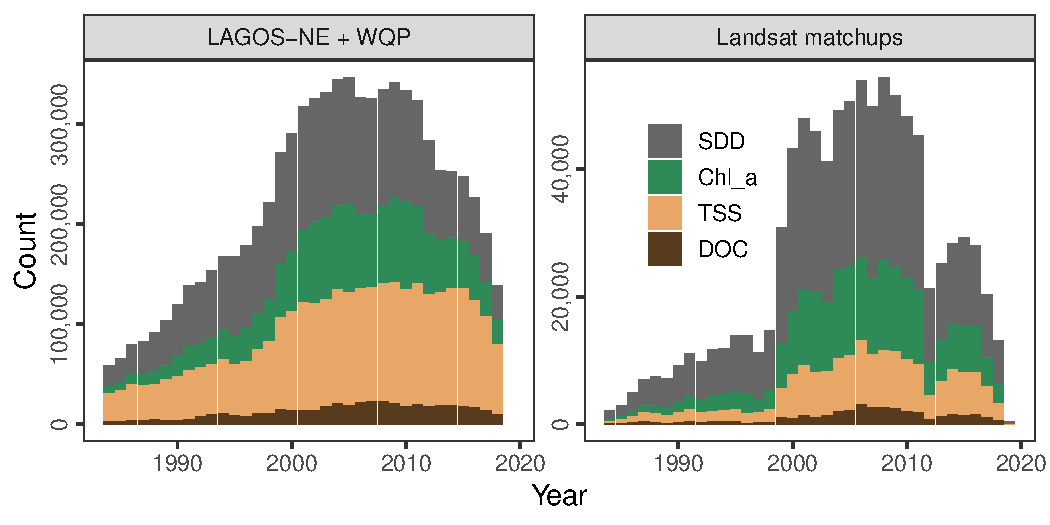
\includegraphics{aquasat_outline_files/figure-latex/time-1.pdf}
\caption{\label{fig:time} Shows the number of observations per year per
parameter type. Note the different y axes, highlighting roughly an order
of magnitude less matchup data than incoming data.}
\end{figure}

The spatial distribution of data shown in figure \ref{fig:map}
highlights how lakes dominate the matchup dataset contributing 76.5\% of
the data to the entire dataset, most of that coming from the secchi
data. Beyond the general trends of what regions are best represented in
the data, it is useful to know the number of observations at a given
site. Figure \ref{fig:distribution} shows the breakdown of overpasses at
a given site and it highlights an important caveat to this dataset. The
vast majority of sites have less than ten matchups, making it unlikely
that one can rely on a single site to build, test, and validate a model
that uses reflectance to predict water quality parameters. However,
there are thousands of sites with at least one observation and if these
sites are close, share the same waterbody or drainage basin, one may be
able to borrow information across sites to have enough data for
modelling/prediction applications. Algthough the majority of sites have
only one overpass, there are several hundred for each parameter that
have at least 50 overpasses, which presents exciting opportunities for
site-specific remote water quality predictions.

The timing of observations in our matchup dataset generally reflect the
availability of data in the WQP and LAGOS-NE and the launching or
retirement of Landsat missions (Fig \ref{fig:time}). The data shown here
lines up well with data reported in the original WQP data paper (Read et
al., 2017). As with fig \ref{fig:distribution}, there is consistently
relatively low amounts of DOC data available throughout the observation
record with much more TSS, Chl\_a, and secchi depth information,
especially in the years from 1999-2012. There is increasing data
available from the start in LAGOS-NE and the WQP through
\textasciitilde{} 2010, with a decline in data thereafter. This decline
may reflect a lag between agencies collecting data and submitting final
datasets to the WQP. The matchup data reflects \emph{in-situ} data
availability while also showing peaks in overpasses when at least two
Landsat satellites are in orbit (late 1990s and post-2013).

\begin{figure}
\centering
\includegraphics{aquasat_outline_files/figure-latex/captured-1.pdf}
\caption{\label{fig:captured} Shows the data distributions for only the
in-situ data in gray with the matchup data distributions in red. Data
quantiles are shown in the background as a color ramp from sage to
blue.}
\end{figure}

The data we captured in the matchup dataset generally reflects the
distribution of \emph{in-situ} data quite well (fig \ref{fig:captured}).
This is especially true for chlorophyll a and secchi disk depth, where
the overpass distribution shapes are nearly identical to the
\emph{in-situ} distributions, with just fewer observations. In both DOC
and TSS data, the matchup data misses the long tails of these
distributions (the highest TSS data and the highest and lowest DOC
data). If we examine which sites are missing in the overpass dataset, we
see that almost all of them are small streams, reflecting higher
variation in TSS and DOC in small streams that gets muted as small
stream signals mix to form larger river, more muted signals
({\textbf{???}}). For all parameters the observations captured span
several orders of magnitude and capture environmentally meaningful
variation in water clarity and quality. Across all parameters the data
is approximately log-normally distributed, with the majority of the data
occupying a relatively narrow range for each parameter (fig
\ref{fig:captured}). This distribution shape, means that the bottom 5
and the top 95th percentiles capture more variation in concentration
than data in the 5-95\% quantiles, reflecting a dataset that does
capture large variation, but where the majority of observations are
restricted to narrow bands. However, these narrow ranges of parameter
values reflect the general distributions in the full WQP and LAGOS-NE
datasets, meaning our data can reasonably be expected to reflect the
overwhelming majority of environmental variation in water quality
parameter concentration.

Based on decades of previous research {[}Topp2018{]}, we know that the
concentration of our four primary parameters should control, to some
degreee, the reflectance from a waterbody that reaches the Landsat
sensor. While exploring these relationships at individual sites or
regions is beyond the scope of this paper, we can interrogate the
dataset to make some initial statements about how variation in each
water quality consitituent maps to variation in reflectance in each
band. To explore these relationships, we divide the data into the six
quantiles shown in (fig \ref{fig:captured}) for each water quality
parameter. We then plot a boxplot of the spectral response within each
data quantile for each spectral band as shown in figure
\ref{fig:variation}. This plot shows how increasing concentrations of
Chlorophyll a, DOC, and TSS or increasing secchi disk depth control
spectral variation across our three waterbody types (Estuary, Stream,
and Lake) and averaged for the entire USA. Despite using such a
heterogeneous dataset, figure \ref{fig:variation} shows clear systematic
variation in spectral response for each parameter as concentration
increases.

Previous work on remote sensing of Chlorophyll a has frequently shown
that the green band frequently is most predictive of Chlorophyll a
concentrations along with the red and NIR bands for exceptionally high
concentrations {[}Topp2018{]}. Our dataset confirms this result, by
showing the largest spectral distinction between chlorophyll quantiles
in the green, red, and NIR bands respectively, with increasing
reflectance with increasing concentration (fig \ref{fig:captured}.
Secchi disk depth and TSS show even stronger responses in the green,
red, and NIR bands, which is also consistent with previous research. TSS
has the notably strongest response, potentially indicating it is one of
the easiest parameters to predict with remote sensing data
{[}Topp2018{]}. In contrast to these three parameters which all have a
single directional response (increasing concentration = increasing
reflectance), the DOC response is more mixed. With increasing
concentrations of DOC, the spectral response is actually muted which is
consistent with the general phenomena of CDOM absorbing light and
reducing reflectance, especially in the gren and red bands
{[}Topp2018{]}. While previous researchers have frequently used the
shortwave infrared bands for remote sensing of water quality, our data
indicates that such data may only be useul at the very highest sediment
and DOC concentrations. These consistent and sensible responses for each
quantile provide some evidence that our dataset will provide a hitherto
unavailable playground for the development, deployment, and distribution
of remote sening of water quality algorithms.

\hypertarget{discussion}{%
\section{Discussion}\label{discussion}}

\begin{figure}
\centering
\includegraphics{aquasat_outline_files/figure-latex/variation-1.pdf}
\caption{\label{fig:captured} Shows spectral response for each data
quantile for each Landsat band. For chl\_a, doc, and tss, concentration
increases moving from left to right for higher quantiles. For secchi
disk dept quantiles mean increasing clarity or increasing depth.}
\end{figure}

Our matchup data generally captures the distribution of \emph{in-situ}
data and spectral responses at a course level show consistent and
predictable relationships between concentration and spectral response.
However, this data comes with plenty of caveats and limitations. First
and foremost, the Water Quality Portal and LAGOS-NE have inherent
spatial biases in terms of which water bodies were sampled, which
agencies fully report their data, and the completeness of records.
Investigating these shortcomings is beyond the scope of this paper, but
end-users should be aware of these inherent pitfalls. Furthermore, our
efforts to harmonize and unify the data in the Water Quality Portal were
primarily with the explicit goal of including as much data as could be
reasonably included. For example, we kept all data that did not have
sampling depth information. This means we cannot gurantee that
\emph{in-situ} concentrations represent surface water quality which is
reflected in Landsat imagery, rather than deeper waters which would not
be captured by satellite imagery. This is a single example of the many
inclusive decisions we made when trimming and harmonizing the WQP data
(Supplement Link). Such inclusivity ensured a dataset that preferenced
quantity over quality gurantees, despite our best efforts to also ensure
data quality. The LAGOS-NE dataset provides a nice foil to our WQP
data-cleaning approach, because the LAGOS-NE dataset has been much more
intensively and carefully harmonized for analysis (Soranno et al.,
2017). Our inclusive approach did not stop at the harmonizing step, we
also elected to keep all data that had positive values. This means we
did not do any quality analysis based on ``sensible'' data values. For
example, there are some secchi disk depth samples that report a secchi
disk depth of \textgreater{} 100s of meters. Such values are highly
unlikely, but we elected to keep them so that end-users can set their
own ``sensibility'' thresholds based on expert knowledge for their
systems. The quality controls we considered in the WQP differs sharply
from our approach with the LAGOS-NE data and the Landsat data. For both
of these data sources, we essentially took the datasets as intact and
analysis-ready with little direct manipulation. This is particularly
important for the Landsat data which we only linked to a single
atmospheric correction for each satellite (LEDAPS for Landsat 5 and 7,
and LaSRC for Landsat 8) or linked to uncorrected top-of-atmosphere
reflectance. There are many papers and review papers, exclusively
devoted to the correct atmospheric correction to use when attempting to
predict water quality concentrations from remote imagery {[}Topp2018{]},
so our data represents a dramatic simplification of this rich research
on atmospheric corrections. As with our WQP data quality choices, we
chose to be inclusive with the Landsat data, by including data that the
Landsat quality assessment bands declared to be ice and/or land, not
simply keeping pixels that are only declared water. This approach allows
us to keep data for the highest TSS concentrations, which can falsely be
declared as ice or land, but it also increases the likelihood that our
spatial medians may be a spoiled pixel that really contains ice or land.
In addition to the data quality checks we chose to do and not do, we
also made the explicit choice to pair imagery with \emph{in-situ}
observations within one day of a satellite overpass. There is ample
research suggesting this assumption works for lakes (Torbick et al.,
2013,@Olmanson2011) (Simon can you add more refs here) and for some
river conditions (Griffin et al., 2011). However, in rapidly changing
river conditions and for estuarine environments our one-day window is
likely too permissive and should be interrogated by end-users. To enable
this kind of \emph{post-hoc} quality check, we have included the time
difference between overpass and water quality sampling in the dataset.
Because this project included a series of essentially user-specific
choices, we are publishing all code, supplemental data, and adjacent
analyses. We hope that publishing the source code for this project will
allow users to define their own rules for data quality assurance, data
inclusivity, and any changes they wish to make. Ideally, for an
experienced R user, re-working these decisiosn will not be incredibly
time-insenstive and one can generate datasets that are complimentary to
our own. To our knowledge and despite the limitations, tradeoffs, and
caveats inherent this dataset, it is still the largest single record of
matchups between \emph{in-situ} observations and remote imagery ever
assembled. We anticipate that such a large dataset, covering most of the
USA, can be used in research at the local, regional, and global scale to
ultimately model and predict water quality from satellite observations.
We hope that by publishing this data, we will further enable the current
transition in the field from developing methods to a field where those
methods are used to interrogate patterns in water quality, drivers of
change, and spatial variability of key water quality parameters
{[}Topp2018{]}. We also have the aim of publishing our data and code
architecture to encourage others to explore remote sensing of different
water quality parameters (like phosphorous or total organic carbon),
additional sites (including coastal environments or other countries),
and even adding new observations paired with public satellites (like
Sentinel 2) or private satellites (like DigitalGlobe or PLANET).

\begin{center}\rule{0.5\linewidth}{\linethickness}\end{center}

\hypertarget{references}{%
\section*{References}\label{references}}
\addcontentsline{toc}{section}{References}

\hypertarget{refs}{}
\leavevmode\hypertarget{ref-Antoine1996}{}%
Antoine, D., André, J.-M., \& Morel, A. (1996). Oceanic primary
production: 2. Estimation at global scale from satellite (Coastal Zone
Color Scanner) chlorophyll. \emph{Global Biogeochemical Cycles},
\emph{10}(1), 57--69. \url{https://doi.org/10.1029/95GB02832}

\leavevmode\hypertarget{ref-Blondeau-Patissier2014}{}%
Blondeau-Patissier, D., Gower, J. F., Dekker, A. G., Phinn, S. R., \&
Brando, V. E. (2014). A review of ocean color remote sensing methods and
statistical techniques for the detection, mapping and analysis of
phytoplankton blooms in coastal and open oceans. \emph{Progress in
Oceanography}, \emph{123}, 23--144.
\url{https://doi.org/10.1016/j.pocean.2013.12.008}

\leavevmode\hypertarget{ref-Brando2003}{}%
Brando, V., \& Dekker, A. (2003). Satellite hyperspectral remote sensing
for estimating estuarine and coastal water quality. \emph{IEEE
Transactions on Geoscience and Remote Sensing}, \emph{41}(6),
1378--1387. \url{https://doi.org/10.1109/TGRS.2003.812907}

\leavevmode\hypertarget{ref-Bukata2013}{}%
Bukata, R. P. (2013). Retrospection and introspection on remote sensing
of inland water quality: "Like Déjà Vu All Over Again". Elsevier B.V.
\url{https://doi.org/10.1016/j.jglr.2013.04.001}

\leavevmode\hypertarget{ref-Butman2016}{}%
Butman, D., Stackpoole, S., Stets, E., McDonald, C. P., Clow, D. W., \&
Striegl, R. G. (2016). Aquatic carbon cycling in the conterminous United
States and implications for terrestrial carbon accounting.
\emph{Proceedings of the National Academy of Sciences}, \emph{113}(1),
58--63. \url{https://doi.org/10.1073/pnas.1512651112}

\leavevmode\hypertarget{ref-Carlson1977}{}%
Carlson, R. E. (1977). A trophic state index for lakes1. \emph{Limnology
and Oceanography}, \emph{22}(2), 361--369.
\url{https://doi.org/10.4319/lo.1977.22.2.0361}

\leavevmode\hypertarget{ref-Caselles1989}{}%
Caselles, V., \& Lóópez Garc Ĺ A, M. J. (1989). An alternative simple
approach to estimate atmospheric correction in multitemporal studies.
\emph{International Journal of Remote Sensing}, \emph{10}(6),
1127--1134. \url{https://doi.org/10.1080/01431168908903951}

\leavevmode\hypertarget{ref-Clarke1970}{}%
Clarke, G. L., Ewing, G. C., \& Lorenzen, C. J. (1970). Spectra of
Backscattered Light from the Sea Obtained from Aircraft as a Measure of
Chlorophyll Concentration. \emph{Science}, \emph{167}(3921), 1119--1121.
\url{https://doi.org/10.1126/science.167.3921.1119}

\leavevmode\hypertarget{ref-Doxani2018}{}%
Doxani, G., Vermote, E., Roger, J.-C., Gascon, F., Adriaensen, S.,
Frantz, D., et al. (2018). Atmospheric Correction Inter-Comparison
Exercise. \emph{Remote Sensing}, \emph{10}(3), 352.
\url{https://doi.org/10.3390/rs10020352}

\leavevmode\hypertarget{ref-Feldman1979}{}%
Feldman, S. I. (1979). Make --- a program for maintaining computer
programs. \emph{Software: Practice and Experience}, \emph{9}(4),
255--265. \url{https://doi.org/10.1002/spe.4380090402}

\leavevmode\hypertarget{ref-Gholizadeh2016}{}%
Gholizadeh, M., Melesse, A., \& Reddi, L. (2016). A Comprehensive Review
on Water Quality Parameters Estimation Using Remote Sensing Techniques.
\emph{Sensors}, \emph{16}(8), 1298.
\url{https://doi.org/10.3390/s16081298}

\leavevmode\hypertarget{ref-Gordon1997}{}%
Gordon, H. R. (1997). Atmospheric correction of ocean color imagery in
the Earth Observing System era. \emph{Journal of Geophysical Research:
Atmospheres}, \emph{102}(D14), 17081--17106.
\url{https://doi.org/10.1029/96JD02443}

\leavevmode\hypertarget{ref-Gorelick2017}{}%
Gorelick, N., Hancher, M., Dixon, M., Ilyushchenko, S., Thau, D., \&
Moore, R. (2017). Google Earth Engine: Planetary-scale geospatial
analysis for everyone. \emph{Remote Sensing of Environment}, \emph{202},
18--27. \url{https://doi.org/10.1016/j.rse.2017.06.031}

\leavevmode\hypertarget{ref-Griffin2011}{}%
Griffin, C. G., Frey, K. E., Rogan, J., \& Holmes, R. M. (2011). Spatial
and interannual variability of dissolved organic matter in the Kolyma
River, East Siberia, observed using satellite imagery. \emph{Journal of
Geophysical Research: Biogeosciences}, \emph{116}(3), 1--12.
\url{https://doi.org/10.1029/2010JG001634}

\leavevmode\hypertarget{ref-Holyer1978}{}%
Holyer, R. J. (1978). Toward universal multispectral suspended sediment
algorithms. \emph{Remote Sensing of Environment}, \emph{7}(4), 323--338.
\url{https://doi.org/10.1016/0034-4257(78)90023-8}

\leavevmode\hypertarget{ref-Ju2012}{}%
Ju, J., Roy, D. P., Vermote, E., Masek, J., \& Kovalskyy, V. (2012).
Continental-scale validation of MODIS-based and LEDAPS Landsat ETM+
atmospheric correction methods. \emph{Remote Sensing of Environment},
\emph{122}, 175--184. \url{https://doi.org/10.1016/J.RSE.2011.12.025}

\leavevmode\hypertarget{ref-Julian2008}{}%
Julian, J. P., Doyle, M. W., Powers, S. M., Stanley, E. H., \& Riggsbee,
J. A. (2008). Optical water quality in rivers. \emph{Water Resources
Research}, \emph{44}(10), 1--19.
\url{https://doi.org/10.1029/2007WR006457}

\leavevmode\hypertarget{ref-Klemas1973}{}%
Klemas, V., Borchardt, J. F., \& Treasure, W. M. (1973). Suspended
sediment observations from ERTS-1. \emph{Remote Sensing of Environment},
\emph{2}, 205--221. \url{https://doi.org/10.1016/0034-4257(71)90094-0}

\leavevmode\hypertarget{ref-Kutser2004}{}%
Kutser, T. (2004). Quantitative detection of chlorophyll in
cyanobacterial blooms by satellite remote sensing. \emph{Limnology and
Oceanography}, \emph{49}(6), 2179--2189.
\url{https://doi.org/10.4319/lo.2004.49.6.2179}

\leavevmode\hypertarget{ref-Lorenzen1980}{}%
Lorenzen, M. W. (1980). Use of chlorophyll-Secchi disk relationships.
\emph{Limnology and Oceanography}, \emph{25}(2), 371--372.
\url{https://doi.org/10.4319/lo.1980.25.2.0371}

\leavevmode\hypertarget{ref-Loveland2012}{}%
Loveland, T. R., \& Dwyer, J. L. (2012). Landsat: Building a strong
future. \emph{Remote Sensing of Environment}, \emph{122}(October 2000),
22--29. \url{https://doi.org/10.1016/j.rse.2011.09.022}

\leavevmode\hypertarget{ref-Maul1975}{}%
Maul, G. A., \& Gordon, H. R. (1975). On the Use of the Earth Resources
Technology Satellite ( LANDSAT-1 ) in Optical Oceanography. \emph{Remote
Sensing of Environment}, \emph{4}(C), 95--128.
\url{https://doi.org/10.1016/0034-4257(75)90008-5}

\leavevmode\hypertarget{ref-Olmanson2011}{}%
Olmanson, L. G., Brezonik, P. L., \& Bauer, M. E. (2011). Evaluation of
medium to low resolution satellite imagery for regional lake water
quality assessments. \emph{Water Resources Research}, \emph{47}(9),
1--14. \url{https://doi.org/10.1029/2011WR011005}

\leavevmode\hypertarget{ref-Pekel2016}{}%
Pekel, J.-F., Cottam, A., Gorelick, N., \& Belward, A. S. (2016).
High-resolution mapping of global surface water and its long-term
changes. \emph{Nature}, \emph{540}(7633), 418--422.
\url{https://doi.org/10.1038/nature20584}

\leavevmode\hypertarget{ref-Read2017}{}%
Read, E. K., Carr, L., De Cicco, L., Dugan, H. A., Hanson, P. C., Hart,
J. A., et al. (2017). Water quality data for national-scale aquatic
research: The Water Quality Portal. \emph{Water Resources Research},
\emph{53}(2), 1735--1745. \url{https://doi.org/10.1002/2016WR019993}

\leavevmode\hypertarget{ref-Richardson1996}{}%
Richardson, L. L. (1996). Remote Sensing of Algal Bloom Dynamics.
\emph{BioScience}, \emph{46}(7), 492--501.
\url{https://doi.org/10.2307/1312927}

\leavevmode\hypertarget{ref-Ritchie1976}{}%
Ritchie, J., Schiebe, F., \& McHENRY, J. (1976). Remote sensing of
suspended sediments in surface waters. \emph{American Society of},
\emph{42}(12), 1539--1545. Retrieved from
\url{https://trid.trb.org/view.aspx?id=66674}

\leavevmode\hypertarget{ref-Robbins2017}{}%
Robbins, C. J., King, R. S., Yeager, A. D., Walker, C. M., Back, J. A.,
Doyle, R. D., \& Whigham, D. F. (2017). Low-level addition of dissolved
organic carbon increases basal ecosystem function in a boreal headwater
stream. \emph{Ecosphere}, \emph{8}(4), e01739.
\url{https://doi.org/10.1002/ecs2.1739}

\leavevmode\hypertarget{ref-Rode2016}{}%
Rode, M., Wade, A. J., Cohen, M. J., Hensley, R. T., Bowes, M. J.,
Kirchner, J. W., et al. (2016). Sensors in the Stream: The
High-Frequency Wave of the Present. \emph{Environmental Science \&
Technology}, \emph{50}(19), 10297--10307.
\url{https://doi.org/10.1021/acs.est.6b02155}

\leavevmode\hypertarget{ref-Secchi1864}{}%
Secchi, P. (1864). Relazione delle esperienze fatte a bordo della
pontificia pirocorvetta l'Immacolata concezione per determinare la
trasparenza del mare; Memoria del P. A. Secchi. \emph{Il Nuovo Cimento},
\emph{20}(1), 205--238. \url{https://doi.org/10.1007/BF02726911}

\leavevmode\hypertarget{ref-Soranno2017}{}%
Soranno, P. A., Bacon, L. C., Beauchene, M., Bednar, K. E., Bissell, E.
G., Boudreau, C. K., et al. (2017). LAGOS-NE: A multi-scaled geospatial
and temporal database of lake ecological context and water quality for
thousands of US lakes. \emph{GigaScience}, \emph{6}(12), 1--22.
\url{https://doi.org/10.1093/gigascience/gix101}

\leavevmode\hypertarget{ref-Sprague2017}{}%
Sprague, L. A., Oelsner, G. P., \& Argue, D. M. (2017). Challenges with
secondary use of multi-source water-quality data in the United States.
\emph{Water Research}, \emph{110}, 252--261.
\url{https://doi.org/10.1016/j.watres.2016.12.024}

\leavevmode\hypertarget{ref-Srebotnjak2012}{}%
Srebotnjak, T., Carr, G., Sherbinin, A. de, \& Rickwood, C. (2012). A
global Water Quality Index and hot-deck imputation of missing data.
\emph{Ecological Indicators}, \emph{17}, 108--119.
\url{https://doi.org/10.1016/J.ECOLIND.2011.04.023}

\leavevmode\hypertarget{ref-Stets2012}{}%
Stets, E., \& Striegl, R. (2012). Carbon export by rivers draining the
conterminous United States. \emph{Inland Waters}, \emph{2}(4), 177--184.
\url{https://doi.org/10.5268/IW-2.4.510}

\leavevmode\hypertarget{ref-Storey2005}{}%
Storey, J., Scaramuzza, P., Schmidt, G., \& Barsi, J. (2005). Landsat 7
scan line corrector-off gap filled product development. \emph{PECORA 16
Conference Proceedings, Sioux Falls, South Dakota}, 23--27. Retrieved
from
\href{http://www.asprs.org/a/publications/proceedings/pecora16/Storey\%7B/_\%7DJ.pdf}{http://www.asprs.org/a/publications/proceedings/pecora16/Storey\{\textbackslash{}\_\}J.pdf}

\leavevmode\hypertarget{ref-Torbick2013}{}%
Torbick, N., Hession, S., Hagen, S., Wiangwang, N., Becker, B., \& Qi,
J. (2013). Mapping inland lake water quality across the Lower Peninsula
of Michigan using Landsat TM imagery.
\url{https://doi.org/10.1080/01431161.2013.822602}

\leavevmode\hypertarget{ref-Vahatalo2005}{}%
Vähätalo, A. V., Wetzel, R. G., \& Paerl, H. W. (2005). Light absorption
by phytoplankton and chromophoric dissolved organic matter in the
drainage basin and estuary of the Neuse River, North Carolina (U.S.A.).
\emph{Freshwater Biology}, \emph{50}(3), 477--493.
\url{https://doi.org/10.1111/j.1365-2427.2004.01335.x}

\leavevmode\hypertarget{ref-Wickham2014}{}%
Wickham, H. (2014). Tidy Data. \emph{Journal of Statistical Software},
\emph{59}(10). \url{https://doi.org/10.18637/jss.v059.i10}

\leavevmode\hypertarget{ref-Williams1989}{}%
Williams, G. P. (1989). Sediment concentration versus water discharge
during single hydrologic events in rivers. \emph{Journal of Hydrology},
\emph{111}(1-4), 89--106.
\url{https://doi.org/10.1016/0022-1694(89)90254-0}

\leavevmode\hypertarget{ref-Williamson2008}{}%
Williamson, C. E., Dodds, W., Kratz, T. K., \& Palmer, M. A. (2008).
Lakes and streams as sentinels of environmental change in terrestrial
and atmospheric processes. \emph{Frontiers in Ecology and the
Environment}, \emph{6}(5), 247--254.
\url{https://doi.org/10.1890/070140}

\leavevmode\hypertarget{ref-Wulder2016}{}%
Wulder, M. A., White, J. C., Loveland, T. R., Woodcock, C. E., Belward,
A. S., Cohen, W. B., et al. (2016). The global Landsat archive: Status,
consolidation, and direction. \emph{Remote Sensing of Environment},
\emph{185}, 271--283. \url{https://doi.org/10.1016/j.rse.2015.11.032}


\end{document}
